\clearpage
\vspace*{\fill}
\begin{figure}[H]
    \centering
      
\includegraphics[width=5cm]{src/cover/title_page_colorspace.png}%
\end{figure}
\vspace*{\fill}
\thispagestyle{empty}%
\clearpage

\chapter{developing a bit of a complex}
\begin{definition}[Jeffrey Says]
\setlength{\intextsep}{0pt}%
\setlength{\columnsep}{3pt}%
\begin{wrapfigure}{l}{0.12\textwidth}

\includegraphics[width=\linewidth]{src/callout/psych.png} 
\end{wrapfigure}
\small
This was the next major evolution of the lightsynth. The Atari machine had a
  much more extensive palette than the Commodore machines, plus you could make
  all kinds of interesting screen modes using the Display List Interrupt
  system, so it seemed like a natural machine to develop a next-generation
  lightsynth on. I still used the same basic algorithm as Psychedelia, but
  introduced a lot more colour variation, and colour cycling. There was also a
  provision for designing static graphics and logos on the screen and having
  the generated patterns flow over or under them, and many more symmetry modes
  afforded by the flexible hardware. Screens could have a cylindrical "curved"
  look since you could vary the vertical pixel size on a scanline by scanline
  basis, thanks to the DLIs.
\end{definition}
Colourspace is a major improvement on its predecessor. As we will see the core is the
same, the algorithms we have covered in detail in Psychedelia remain unchanged, but the hardware of the
Atari 8 bit computers created opportunities for much more colour and complexity.

To me, one of the most impressive things about Colourspace is the speed of its development. Minter
managed to speed through it in a few short months in 1985 while also completing other projects.

In our next chapter we'll take a look at some of the things he had to learn about the Atari and adapt
to the purpose of making a new generation of Psychedelia and this will give us a clear sense of 
the scale of the undertaking in such a short time.


\clearpage
\begin{figure}[H]
    \centering
    \begin{adjustbox}{width=12cm,center}
    \frame{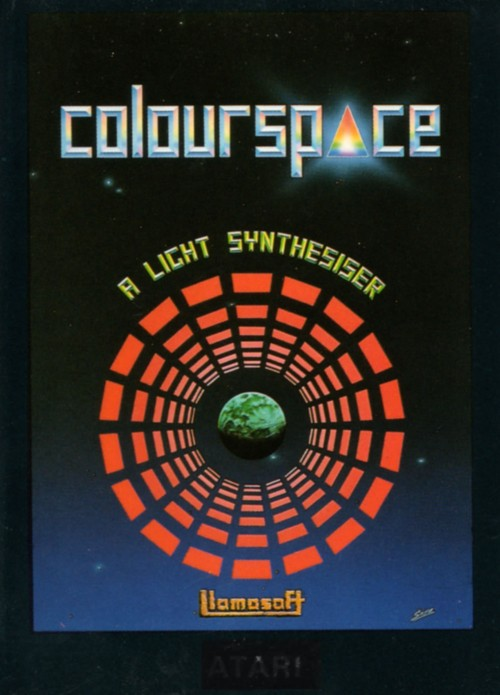
\includegraphics{src/preface_colorspace/colorspace.jpg}}%
    \end{adjustbox}
\caption{Cover art by Steinar Lund for the commercial edition of Colourspace}
\end{figure}
\clearpage
\begin{definition}[Jeffrey Says]
\setlength{\intextsep}{0pt}%
\setlength{\columnsep}{3pt}%
\begin{wrapfigure}{l}{0.12\textwidth}

\includegraphics[width=\linewidth]{src/callout/psych.png} 
\end{wrapfigure}
\small
The resultant program, PSYCHEDELIA, is now available for many popular micros,
and has freaked quite a few people out.  Using keyboard and joystick, operators
can produce lightshows to accompany their favourite music.  The displays have
been described as being like "interactive fireworks".  Whilst satisfying on
their own, the displays are best to the accompanyment of loud music, which acts
like a catalyst and vastly increases the enjoyment of playing.  The system is
set up like a synthesizer, with user-controllable variables defining the modes
of pattern-generation.  Users "perform" using the joystick and can store away
effects for later recall by a single keypress.
This program, COLOURSPACE, is based upon the same basic idea.  By using the
unique Atari screen hardware and colour pallette, the effect of the program is
much improved.  The difference between Psychedelia and Colourspace is as
pronounced as the difference between a Mini and a Ferrari.  Using the Atari you
can get curved screens, hardware reflections, interlace effects, stroboscopics,
dynamic colourflows, and variable resolution screens.  There are 80 presets
available for programming, 16 user-definable lightforms, and a foreground
drawing mode.  There is even a mode which allows you to perform simultaneously
with another player or with the computer.
\end{definition}


